\documentclass[twocolumn]{emulateapj}

\newcommand{\vdag}{(v)^\dagger}
\def\ba{\begin{eqnarray}}
\def\ea{\end{eqnarray}}
\usepackage{graphicx, amsmath, amsthm, amssymb,color}
\newcommand\aastex{AAS\TeX}
\newcommand\latex{La\TeX}
\def\qr#1{{\color{red}{\bf Cristobal: #1}}}
\begin{document}

%%%%%%%%%%%%%%%%%%%%%%%%%%%%%%%%%%%%%%%%%%%%%%%%%%%%%%%%%%%%
% TITLE %
%%%%%%%%%%%%%%%%%%%%%%%%%%%%%%%%%%%%%%%%%%%%%%%%%%%%%%%%%%%%
\title{Title}

%%%%%%%%%%%%%%%%%%%%%%%%%%%%%%%%%%%%%%%%%%%%%%%%%%%%%%%%%%%%
% AUTHOR %
%%%%%%%%%%%%%%%%%%%%%%%%%%%%%%%%%%%%%%%%%%%%%%%%%%%%%%%%%%%%
\author{Emily Deibert}
\author{Chelsea Huang}
\author{Cristobal Petrovich}
%\affil{Dunlap Institute for Astronomy \& Astrophysics, University of Toronto, 50 St. George Street, Toronto, Ontario, M5S 3H4, Canada \href{mailto:emily.deibert@mail.utoronto.ca}{emily.deibert@mail.utoronto.ca}}

%%%%%%%%%%%%%%%%%%%%%%%%%%%%%%%%%%%%%%%%%%%%%%%%%%%%%%%%%%%%
% ABSTRACT %
%%%%%%%%%%%%%%%%%%%%%%%%%%%%%%%%%%%%%%%%%%%%%%%%%%%%%%%%%%%%
\begin{abstract}
Hundreds of multi-planetary systems have been discovered 
by the Kepler mission, most of which planets  have radii $\lesssim4R_\odot$
and close-in (inside $\sim100$ days)
and low eccentricity and inclination orbits. 
In contrast, the planets discovered in Radial Velocity surveys
(mostly non-transiting giant planets) orbit 
in wider and more eccentric orbits.
We run N-body experiments of planetary systems with 
unstable outer giant planets and inner Kepler-like multi-transit systems
and investigate the possible dynamical links between these
two exoplanet populations.
We find that... 

\end{abstract}

%%%%%%%%%%%%%%%%%%%%%%%%%%%%%%%%%%%%%%%%%%%%%%%%%%%%%%%%%%%%
% KEYWORDS %
%%%%%%%%%%%%%%%%%%%%%%%%%%%%%%%%%%%%%%%%%%%%%%%%%%%%%%%%%%%%
\keywords{planets and satellites: dynamical evolution and stability}

%%%%%%%%%%%%%%%%%%%%%%%%%%%%%%%%%%%%%%%%%%%%%%%%%%%%%%%%%%%%
% INTRODUCTION %
%%%%%%%%%%%%%%%%%%%%%%%%%%%%%%%%%%%%%%%%%%%%%%%%%%%%%%%%%%%%
\section{Introduction} \label{sec:intro}
Originally launched in 2009, NASA's \textit{Kepler} mission is responsible for the discovery of thousands of planetary candidates, including over 2000 confirmed planets (\citealt{Morton2016}). Through monitoring periodic changes in brightness of light curves from stars (i.e. the ``transit method''), \textit{Kepler} is able to detect planets with radii on the order of 1 $\text{R}_{\oplus}$, although the majority of planets detected are so-called ``super-Earths'' or ``sub-Neptunes'' (with radii $\sim 1.2 - 3 \text{R}_{\oplus}$, \citealt{Lai2016}). Of the thousands of planetary systems discovered by \textit{Kepler} to date, 80\% are single-transit systems (i.e. only one planet is observed to transit), while the other 20\% consist of 2-7 transiting planets (\citealt{Lai2016}). As detailed in \citealt{Johansen2012}, the relative numbers of single- and multi-transit systems are a function of both the intrinsic system multiplicity and mutual inclinations between planets, and for this reason can reveal important information about the architecture of compact planetary systems.

\qr{Is the motivation the Kepler dichotomy or something more general?}
Many studies have explored the underlying planetary system architectures that can account for the relative numbers of single- and multi-transit systems in the \textit{Kepler} data (see, for e.g., \citealt{Lai2016}, \citealt{Johansen2012}, and \citealt{Moriarty2015}); however, models with a single mutual inclination distribution that have been proposed to date have consistently under-predicted the number of single-transit systems as compared with observations---a problem that will henceforth be referred to as the ``\textit{Kepler} dichotomy''. Previous studies into the \textit{Kepler} dichotomy have generally come to the conclusion that the architectures of planetary systems must either vary significantly or have more than one main mode. In this paper, however, we put forth an alternate explanation by which scattering between distant planets with properties drawn from Radial Velocity (RV) surveys can account for the relative numbers of single- and multi-transit systems observed in \textit{Kepler} data. 

There is evidence that at least a fraction of the single-transiting planets in Kepler occupy dynamically hotter orbits.
First, \citet{MW14} find that the obliquity distribution... Second, \citet{dong16} claims that the eccentricity distribution measured from transit durations can be fitted with two populations: 


Our methods involve drawing from observations of both \textit{Kepler} and RV planets in order to simulate systems consisting of a closely-packed (i.e. within 1 AU) inner system of super-Earths and a more distant (i.e. between 2-5 AU) system of Jupiter-like planets. Using the N-body code \texttt{REBOUND} (\citealt{Rein2011}), we evolve a statistically-significant number of such systems over time and report on the mutual inclinations and number of transits of the evolved systems.

This paper will proceed as follows. In section \ref{sec:sims}, we will discuss the details of the code used to run the simulations, as well as the initial conditions chosen to explore the problem. Our results are presented in section \ref{sec:results}, including the effects of different populations and initial conditions used in the simulations. The results are discussed in section \ref{sec:discussion}, and our conclusions are presented in section \ref{sec:conclusion}.  



\begin{figure}[htbp!]
\centering
\includegraphics[width=\columnwidth]{observed_try3.png}
\caption{Known planet systems with long period giant planets and close-in Super Earths ($M{\rm sin}i<0.1\,M_{J}$), color coded by the number of planets in the system. 
\label{fig:observed}}
\end{figure}

\clearpage


\section{Simulations}
\label{sec:sims}
We run N-body simulations of the evolution of the orbits of inner Kepler-like planets and outer giant planets (masses $>0.3M_J$) orbiting a solar-type star. 
Planet–star and planet–planet collisions are assumed to result in momentum-conserving mergers with no fragmentation. Collisions are assumed to happen when the distance between two planets (or planet and star) becomes less than the sum of their physical radii. The merged body is assumed to conserve total mass and volume. 
A planet is ejected from the system when the distance from the center of mass exceed 100\,AU and the eccentricity is larger than 1, or when the distance from the center of mass exceed 1000\,AU. 


\subsection{The code}
\label{sec:code}

We use the publicly available integrator IAS15 
\citep{RS15}, which is a high-order scheme
that is part of REBOUND package \citep{Rein2011}.
 We justify this choice because we 
are mostly interested on the evolution of dynamically active 
systems, where planets experience several close encounters, and 
the IAS15 can handle close encounters with
high precision.

We include the effect from General Relativity in some 
experiments using the package REBOUNDx with the option 
{\it gr-potential} (Tamayo et al., in prep.), which gives 
the right pericenter precession, but gets mean motion wrong by 
$\mathcal{O}(GM/[ac^2])$.


%%%%%%%%%%%%%%%%%%%%%%%%%%%%%%%%%%%%%%%%%%%%%%%%%%%%%%%%%%%%
% INITIAL %
%%%%%%%%%%%%%%%%%%%%%%%%%%%%%%%%%%%%%%%%%%%%%%%%%%%%%%%%%%%%
\subsection{Initial conditions}
\label{sec:init}
%{\bf TBD: divided up}

We initialize our planetary systems with either Super-Earths (the Kepler population) or gas giant planets (Radial Velocity population) so we can match the bulk of their orbital architectures after either population has evolved for $>1$ Myr. We assess the match to the observed orbital properties for the Kepler-like systems and the Radial Velocity population in \S\S\ref{sec:kepler} and \ref{sec:juponly}, respectively.

\subsubsection{Super-Earth population}


We initialize our systems with Super-Earths located inwards of 1\,AU and choose the semimajor axes as follows.
First, we use the fitting function for the probability distribution of semi-major axes in the {\it  Kepler} sample, after accounting for geometric selection effects \citep{TD11}: 
\ba 
dp(a)=0.656 \frac{(a/a_0)^{3.1}} {1+(a/a_0)^{3.6}}
\frac{da}{a}, \quad a<1.15\,\mbox{AU}
\label{eq:epsilon}
\ea 
where $a_0=0.085\,$AU.  
We then generate an initial distribution
in the period ratio $\mathcal{P}$ ($\mathcal{P}>1$) of a two-planet (two neighboring planets)
system by generating two random variables, $\alpha_1$ and $\alpha_2$, from this
probability distribution and computing
$\mathcal{P}=\max\left\{(\alpha_1/\alpha_2)^{3/2}, (\alpha_2/\alpha_1)^{3/2}\right\}$.
Repeated independent realizations of $\mathcal{P}$ generates a smooth initial distribution in period ratio between neighboring planets are shown in Figure \ref{fig:init-pratio}, which roughly matches to the observed one from {\rm Kepler}. We further limit the period ratio between any outer planet and its neighboring inner planet to be $1.4<\mathcal{P}<5$ so we avoid both systems that can become unstable in relatively short timescales ($<1$ Myr) at $\mathcal{P}<1.4$ and too widely separated planet pairs.
The distribution of period ratio between neighboring planets are shown in Figure \ref{fig:init-pratio}, which roughly matches to the observed one from {\rm Kepler}.

Second, we place the inner planet at $a_1=0.1$ AU (\qr{true?}) and the (i+1)-th planets, where $i$ is in order of increasing semi-major axes, following
\ba
a_{i+1}=a_{i}\mathcal{P}^{-2/3},
\ea
where $\mathcal{P}$ is an independent realization of the period ratio from the procedure discussed above. 


The planets have non-zero eccentricities $e$
and/or inclinations $i$. These are assumed to be randomly distributed following a Rayleigh law, 
\ba
dp=\frac{x\,dx}{\sigma_x^2} \exp\left(-\onehalf x^2/\sigma_x^2\right),
\label{eq:sigma_e}
\ea
where $x=e$ or $i$ and $\sigma_x$ is an input parameter that
is related to the mean and rms eccentricity or inclination by $\langle
x\rangle=\sqrt{\pi/2}\sigma_x=1.253\sigma_x$, $\langle
x^2\rangle^{1/2}=\sqrt{2}\sigma_x=1.414\sigma_x$.


 The masses of the Super-Earths were either 5, 10, or 15 $\text{M}_{\oplus}$, but the ordering of the masses was randomized. This choice is arbitrary and the range of masses $5-15~\text{M}_{\oplus}$ is characteristic for planets with $\sim2-4~\text{R}_{\oplus}$ (e.g., \citealt{WM14}).

\subsubsection{The gas giant population}

We choose the semi-major axis to be uniformly distributed 
in a defined range 2-5 AU. 
Labeling the planets by subscripts $i$ in order of increasing 
semi-major axis, we impose a minimum initial spacing 
of the orbits given by
\ba
\Delta a_{i,i+1}&\equiv& a_{i+1}-a_{i}>K R_{H,i,i+1},\mbox{where} \nonumber \\
R_{H,i,i+1}&=&\left(\frac{M_i+M_{i+1}}{3 M_\star}\right)^{1/3}
\frac{a_i+a_{i+1}}{2},
\label{eq:delta_a}
\ea
and $R_{H,i,i+1}$ is the mutual Hill radius of planets
with masses $M_i$ and $M_{i+1}$.

The initial spacing between orbits mainly changes the 
timescale of onset of dynamical instability
(e.g., \citealt{CWB96}). 
Our choice of $K$ in Equation (\ref{eq:delta_a}) is
empirically guided by the fact that we would like to avoid very 
closely-packed systems which might be subject to gravitational focusing, leading to a spurious excess of planet-planet collisions. 

We initialize the system with three gas giant planets
and use $K=3$.
For reference, a crude estimate of the instability time
can be obtained from the numerical experiments by  
\citet{CFMS2008} using a different initial spacing law $\Delta a_{i,i+1}=\tilde{K} R_{H,i,i+1}$ 
(i.e., the spacing is a fixed multiple of the Hill radius, rather than 
exceeding a multiple of the Hill radius). 
They show that for a distribution of planet masses in the
range $0.4-4~M_J$ the median instability 
timescale can be fitted by the following expression
\ba
\log_{10} (t/\mbox{orbits})=0.021+0.03\exp(1.1~\tilde{K}),
\label{eq:K_tilde}
\ea
where the orbits are those of the innermost planet. 
By assuming that the spacing is a fixed multiple of the Hill radius and that the planet have Jupiter masses, our range of semi-major axes of $2-5$ AU allows for $\tilde{K}$ in the range $\sim 3-5$ (\qr{check}) meaning instability timescales spans in $\sim10-10^7$ orbits. In practice, our experiments show that the median instability timescale is $\sim xx$ orbits and most (xx\%) systems become unstable after 1 Myr (see the results in \S\rec{sec:juponly}). 

The masses of the Jupiters are uniformly drawn between 0.3 $M_{\rm J}$ and 3 $M_{\rm J}$. These initial conditions are chosen so that our Jupiter like planets will reproduce the radial velocity population (see Section \S \ref{sec:juponly}). 


\begin{figure}[htbp!]
\includegraphics[width=\columnwidth]{Period_ratio.pdf}
\caption{The initial period ratio distribution of neighboring super Earths.
\qr{Add the Kepler-only simulation. I would suggest plotting initial and final only of all neighbors; the distribution itself does not distinguish between $P_2/P_1$ and $P_3/P_2$. Maybe the observations can be added as well.}}
\label{fig:init-pratio}
\end{figure}



%Fig. \ref{fig:mass-init} shows the initial setup of the randomized-mass simulations.

%\begin{figure}[htbp!]
%\includegraphics[width=\columnwidth]{Initial.pdf}
%\caption{The initial plot of orbital eccentricity vs semi-major axis, colour-coded by mass, for the set of simulations where the planets' masses have been randomized.}
%\label{fig:mass-init}
%\end{figure}

%{\bf TBD: need a schematic figure to demonstrate the initial set ups}

%CH: initial condition not important to show
%\begin{figure}[htbp!]
%\centering
%\includegraphics[width=\columnwidth]{newinc-initial.pdf}
%\caption{The initial orbital eccentricity vs semi-major axis for the six planets run.}
%\label{fig:init-e}
%\end{figure}

%\begin{figure}[htbp!]
%\includegraphics[width=\columnwidth]{newinc-initial-inc.pdf}
%\caption{The initial nclination vs semi-major axis for the six planets run.}
%\label{fig:init-i}
%\end{figure}

\begin{figure}[htbp!]
\centering
\includegraphics[width=\columnwidth]{a_e_jup_only.pdf}
\caption{Eccentricity versus semi-major axis of the Jupiter-like planet at the end of 1\,Myr evolution. The planets are colour-coded by the multiplicity of their system.}
\label{fig:mass-final}
\end{figure}



\begin{figure}[htbp!]
\centering
\includegraphics[width=\columnwidth]{ejup_only.pdf}
\caption{The final eccentricities distribution of the Jupiter like planets after 1\,Myr evolution. Black line indicate a Rayleigh distribution with $\sigma_e=0.2$. The initial eccentricity distribution has a Rayleigh width of $\sigma_e=0.01$.}
\label{fig:hist-ecc-jup}
\end{figure}


\begin{figure}[htbp!]
\centering
\includegraphics[width=\columnwidth]{inc_jup_only.pdf}
\caption{The final inclination distribution of the Jupiter like planets after 1\,Myr evolution.
The initial inclination distribution has a Rayleigh width of $\sigma_i=0.01$.
}
\label{fig:hist-inc-jup}
\end{figure}



\section{Results}
\label{sec:results}
\subsection{Kepler-like systems only}
\label{sec:kepler}

We evolved 160 systems of 1 Myr. We find no significant change on the multiplicity and orbital elements $e$ and $i$. 
The distribution can roughly reproduce the spacing and typical eccentricities and mutual inclinations
(fabrycky et al.2014).

The results are expected because the typical mutual Hill spheres have $\sim0.005$ AU and $\sim10$ mutual Hill separations required for stability up to $10^8$ orbits (citations) correspond to
period ratios $\lesssim1.6$, where we have only a small fraction of the systems.

\subsection{The radial velocity population only}
\label{sec:juponly}


\begin{table}[htbp!]
\centering
\begin{tabular}{c  c}
\hline
\hline
$\text{N}_{\text{J}}$ & Percentage of Systems \\
\hline
1 & 19.4 \% \\
2 & 76.2 \% \\
3 & 4.4 \% \\
\hline
\end{tabular}
\caption{Multiplicity distribution of the Jupiter like planets.}
\label{tab:randommass}
\end{table}

We evolve 160 realizations of systems to 1\,Myr. The outcome in Table \ref{tab:randommass} reproduces three planet scattering experiments in the literature (\citep{Petrovich:2014} {\bf more references?}). 
In Fig. \ref{fig:mass-final}, we see that most of systems become unstable, in particular, about 76$\%$ of the systems lost one of its planet at the end of run. About $20\%$ of the systems have only one planet left, due to one collision between the planets with either an ejection or collision with the host star. Only $4.5\%$ of the systems stay relatively inactive, which are expected to become unstable if were evolved for long enough time. We show the eccentricity distribution of giant planets with $a<5$\,AU in Figure \ref{fig:hist-ecc-jup}. The mean eccentricity of these systems are about 0.29, which reproduce the observed eccentricity distribution of planets at $>1$\,AU. Most of the systems have relatively low inclination, with a median inclination of 6 degrees (Figure \ref{fig:hist-inc-jup}). 

%CH: does not need the final mass figures. 
%\begin{figure}[htbp!]
%\centering
%\includegraphics[width=\columnwidth]{Final-Mass.pdf}
%\caption{The final eccentricities vs semi-major axes of the surviving planets. Planets are colour-coded by their masses.}
%\label{fig:mass-final-mass}
%\end{figure}







%CH: we can use the table only for this:
%\begin{figure}[htbp!]
%\includegraphics[width=\columnwidth]{NJupiters.pdf}
%\caption{A histogram of the number of planets remaining in the 160 simulated systems after 1 Myr of integration. Note that these are the systems for which the initial masses of the planets were randomized.}
%\label{fig:mass-histogram}
%\end{figure}

\begin{figure}[htbp!]
%\includegraphics[width=\columnwidth]{newinc-multiplicity.pdf}
\includegraphics[width=\columnwidth]{Fiducial/a_e_nplanet.pdf}
\caption{Orbital eccentricity vs semi-major axis for the fiducial run, color-coded by system multiplicity. Jupiter like planets are represented by circles, while Super Earths are represented by diamonds.}
\label{fig:multiplicity}
\end{figure}
\begin{figure}[htbp!]
%\includegraphics[width=0.9\columnwidth]{newinc-nearths.pdf}
\includegraphics[width=\columnwidth]{Fiducial/a_e_nearth.pdf}
\caption{Similar to Figure \ref{fig:multiplicity}, while the planets are color coded by the number of Super Earths in the system.}
\label{fig:nearths}
\end{figure}
\begin{figure}[htbp!]
%\includegraphics[width=0.9\columnwidth]{newinc-njupiters.pdf}
\includegraphics[width=\columnwidth]{Fiducial/a_e_njup.pdf}
\caption{Similar to Figure \ref{fig:multiplicity}, while the planets are color coded by the number of Jupiters in the system.}
\label{fig:njupiters}
\end{figure}

\begin{figure}[htbp!]
\includegraphics[width=\columnwidth]{Fiducial/a_i_nearth.pdf}
\caption{Orbital inclination vs semi-major axis for the fiducial run, color-coded by number of Super Earths in the system. Jupiter like planets are represented by circles, while Super Earths are represented by diamonds.}
\label{fig:inc}
\end{figure}

%%%%%%%%%%%%%%%%%%%%%%%%%%%%%%%%%%%%%%%%%%%%%%%%%%%%%%%%%%%%
% RESULTS %
%%%%%%%%%%%%%%%%%%%%%%%%%%%%%%%%%%%%%%%%%%%%%%%%%%%%%%%%%%%%
\subsection{The Super-Earth and gas giant populations together} \label{sec:standardrun}

Having characterized both the Kepler and Radial Velocity populations independently, we now turn to our main experiment, namely putting both populations together.

We first describe the results for our fiducial simulation. In this simulation we set up systems with initially 3 Super Earths and 3 Jupiters, while the 
eccentricities and inclinations of all the planets were drawn from Rayleigh distribution in Equation (\ref{eq:sigma_e}) with $\sigma_e=0.01$, and $\sigma_i=0.01 \,{\rm rad}$. 

We evolve the fiducial run for xxx realizations till 1\,Myr. The systems are initialized with eccentricities and inclinations draw from a Rayleigh distribution with $\sigma_e, \sigma_i=0.01$. The outcomes are listed in Table \ref{tab:results}.
Figs. \ref{fig:multiplicity}, \ref{fig:nearths}, and \ref{fig:njupiters} show the eccentricity versus semi-major axis of all the remaining planets at the end of 1\,Myr, color-coded by system multiplicity, number of remaining Super-Earths, and number of remaining Jupiters, respectively. Figure \ref{fig:inc} show the inclination versus semi-major axis of all the remaining planets at the end of 1\,Myr, color coded by number of remaining Super-Earths. We detailed the various outcomes as the following: 

\begin{itemize}
\item {\bf No Super Earths:} slightly less than half of the system ($47 \%$) resulted in that the scattering of giant planets disrupt the inner Super Earths completely, leaving mostly two eccentric Jupiter like those in typical RV systems. 

\item {\bf Super Earths with Giant planets:} most of the other half ($49\%$) of the systems lost at least one giant planet due to either ejection or scattering, stir up the close-in Super Earths but do not destroy all of them.
\begin{itemize}

\item The systems with one, two and three Super Earths remaining together with two giant planets are about 16, 3, and 14 percent of the total outcomes. The remaining single Super Earths almost always have high eccentricity and inclination. They typically have a flat eccentricity distribution from 0.1 to as high as 0.8, and inclination as high as 60 degrees. The systems with two Super Earths remaining have eccentricity between 0.1-0.4. A fraction of the three Super Earths systems have modest eccentricity between 0.1-0.2, and inclination between 10-20 degree. If a collision happen between the giant planets instead of an ejection, the Super Earths remain dynamically cold. 

\item About $7\%$ of the systems have one eccentric Jupiter left with dynamically hot Super Earths systems. Since the eccentricity distribution of the single Jupiter is similar to those of the inner planet of the two Jupiter systems, the properties of Super Earths are almost indistinguishable from those have two Jupiters.

\end{itemize}

\item {\bf Inactive:} only $3\%$ have all six planets at the end of run. These systems are expected to become unstable in longer time scale. 

\end{itemize}



We take a more detailed look at the systems that lost at least one planet and still with super Earths remaining. The inclinations and eccentricities of the systems with one/two/three Super Earths are shown in Figure \ref{fig:inc_earthonly}. They follow the trend of xxx. In general, systems with less Super-Earths have higher eccentricity and higher inclination. We show the comparison of our systems to the Kepler single and multiple systems. As derived by \cited{Xieetal:2016}, the Kepler single planet systems can be modeled by an eccentricity distribution with Rayleigh width $\sigma_e=0.32\pm0.023$, while the multiple systems are much more circular, with an eccentricity uplimit at $\sim0.07$. We fit the eccentricity and inclination distribution for our single Super Earth population with a Rayleigh distribution, and obtain that the Rayleigh width to be $\sigma_e=0.37$ and $\sigma_i=20^{\circ}$. This is expected to be more eccentric than the observed single population since the observed population is contaminated by some of the dynamically cold multiple systems with only one planet transit. 

\begin{figure*}[htbp!]
\centering
\includegraphics[width=\linewidth]{Fiducial/i_e_nearth_observe.pdf}
\caption{Orbital inclination versus eccentricity for the systems with Super Earths survive, color coded by the number of Super Earths in the system. We show the linear trend $e=i$ and $e=2i$ to compare with. We also show the location of Kepler multiple systems (red) and single systems (cyan) on this plane as derived by \cited{Xieetal:2016}. The inclination of the Kepler single systems are assumed to be the same as their derived eccentricity. Kepler-56 system is noted as the green dot with the inclination taken from the measurement from the gravitational mode of the host star \cited{Huber:2013}, and eccentricity taken from the dynamic estimation from \cited{Huber:2013} assuming a low mutual inclination between the close-in planets.
\label{fig:inc_earthonly}
}
\end{figure*}

There are a few exceptions to this trend, with the Super-Earths being roughly circular, while the inclinations are as high as 50 degrees. We have identified these systems as the class of ``misaligned multiples", such as Kepler-56, with low mutual inclinations between the Super-Earths. We demonstrate the time evolution of one of this system in Figure \ref{fig:orbit_tilt}. In this example, the ejection of planet 2 at 0.2\,Myr has tilted the orbital plane of all the three Super Earths all together, leading to their inclinations oscillate between 30 to 90 degrees. 


\begin{figure*}[htbp!]
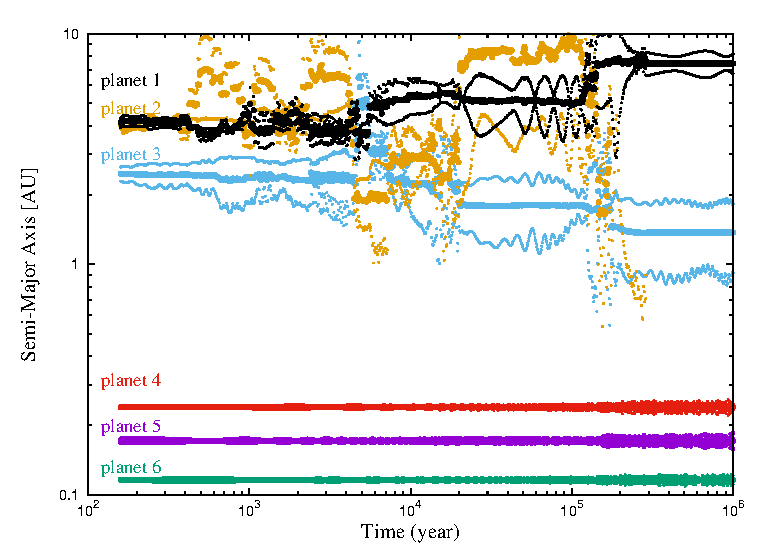
\includegraphics[width=\columnwidth]{GR/orbit_tilt_e.eps}
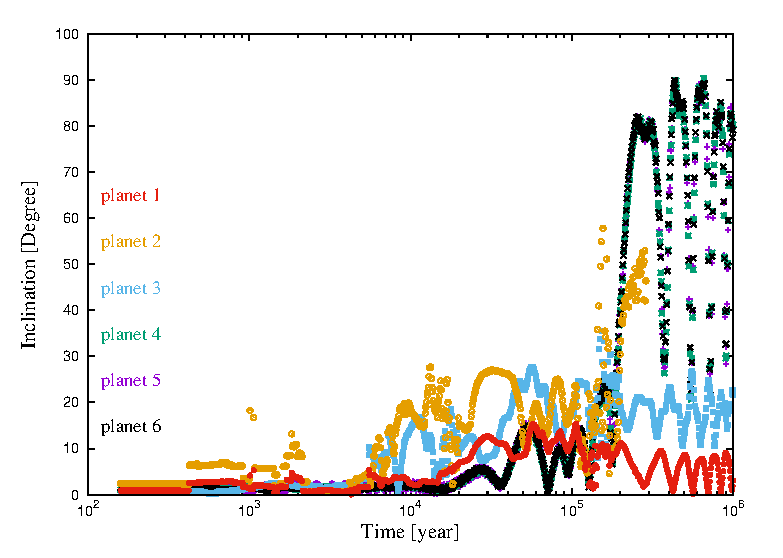
\includegraphics[width=\columnwidth]{GR/orbit_tilt_i.eps}
\caption{Time evolution of a realization of our simulation which resemble the Kepler-56 system. The left panel shows how the semi major axis (thick lines), pericenter (thin lines) and apocenter (thin lines) of 6 planets vary in 1\,Myr. The right panel shows the inclination of all the planets in degrees. One of the giant planet (planet 2) is ejected at 0.2\,Myr. At the end of 1\,Myr, This system has three roughly coplanar and circular Super-Earths (planet 4,5 and 6) with two eccentric giant planets (planet 1 and 3), while the inclination of the Super-Earths oscillate between 30 to 90 degrees. 
\label{fig:orbit_tilt}}
\end{figure*}

We also identified the giant planets with semi major axis smaller than 5 AU, and compare their eccentricities in Figure \ref{fig:ejup_nearth}. We report that only Jupiters with eccentricity smaller than 0.7 can keep Super-Earths in the system. The lower eccentricity the Jupiters have, it is more likely to allow higher multiplicity Super-Earths systems to survive. Most of the three Super-Earths system are likely to be found around Jupiters with eccentricity smaller than 0.3. 

%{\bf TBD: make evolution figures for systems with one/two/three Super Earths left.}
%We demonstrate the time evolution of a xxx like system {\it CH: (a real system we like)} in Figure xxx. 

Finally, we used the code \texttt{CORBITS} \citep{Brakensiek:2016} to determine the effect of scattering on the transit probability of Super-Earths in the remaining systems. This is presented in Figure. \ref{fig:transits}. As can be seen, the number of single-transit systems roughly doubles after 1 Myr of evolution of the systems. While the ratio between the two transit and three transit system stayed roughly the same, the ratio between the signal transit system and the two planet system increased to be a factor of 3.5. 






\begin{figure*}
\includegraphics[width=\columnwidth]{Fiducial/e_jup_nearth.pdf}
\includegraphics[width=\columnwidth]{Fiducial/e_jup_nearth_2Myr.pdf}
\caption{The cumulative histogram of eccentricities for giant planets within $a<5$ AU with super earths in the same system.
\label{fig:ejup_nearth}}
\end{figure*}


\begin{figure}[htbp!]
\includegraphics[width=\columnwidth]{Newinclination/transits.pdf}
\caption{The probability of observing 1, 2, or 3 Super-Earth transits with the $\sigma_i=1^{\circ}$ run. Purple histogram shows initial conditions, and orange histogram shows after 1\,Myr.}
\label{fig:transits}
\end{figure}


\begin{table}[htbp!]
\centering
\begin{tabular}{c c c c c}
\hline
\hline
($\text{N}_{\text{J}}$, $\text{N}_{\text{SE}}$) & fiducial run & $\sigma_i=1^{\circ}$ & GR & 2\,Myr\\
\hline
(1, 0) & 10\% & 9\% & 6\% & 14\%\\
(1, 1) & 4\% & 3\%  & 3\% & 5\%\\
(1, 2) & 0\% & 1\% & 1\% & 1\% \\
(1, 3) & 2\% & 1\% & 3\% & 3\%\\
(2, 0) & 32\% & 38\% & 25\% & 34\%\\
(2, 1) & 11\% & 14\% & 18\% & 13\%\\
(2, 2) & 11\% & 3\% & 6\% & 8\%\\
(2, 3) & 23\% & 22\% & 34\% & 18\%\\
(3, 0) & 2\% & 3\% & 1\% & 0\%\\
(3, 1) & 1\% & 1\% & 0\% & 0\%\\
(3, 2) & 0\% & 0\% & 0\% & 0\%\\
(3, 3) & 4\% &  3\% & 3\% &4\% \\
\hline
\end{tabular}
\caption{End status distribution.}
\label{tab:results}
\end{table}

\subsection{Effect of General Relativity}

We study the effect of general relativity here and how they limit the eccentricity growth of the Super Earths. We do this by using the post newtonian correction term ... ({\bf TBD:elaborate}). The effect of add in the general relativity term are demonstrated in Figure \ref{fig:GRexample}.  

\begin{figure}[htbp!]
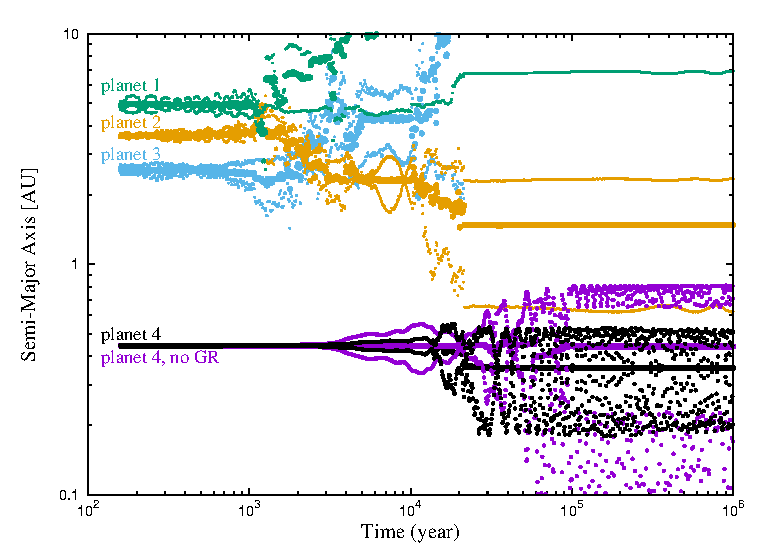
\includegraphics[width=\columnwidth]{GRexample.eps}
\caption{Semi major axis (thick line), pericenter and apocenter (thin lines) of planets over time with the general relativity potential taken into account. The system start with 6 planets, with planet 1, 2 and 3 to be Jupiter like planets, and planet 4,5,6 to be close-in Super Earths. Planet 5 and 6 were ejected around $10^4$\,yrs, and are not shown in the plot. The purple curve shows the survived Super Earth (planet 4) has a modest eccentricity of about 0.4. For comparison, the green curve shows the evolution of planet 4 without the general relativity effect. The planet's eccentricity can growth to as high as 0.8 and will eventually collide with the host star without taken into account of GR.  
\label{fig:GRexample}}
\end{figure}

We simulated 160 realization with the effect of GR, and the detailed outcomes are shown in Table \ref{tab:results}. While the demographic of outcomes do not change dramatically, the percentage of systems with Super Earths at the end of 1\,Myr increased from $56\%$ to $68\%$. This increase most comes from the higher survival rate of single Super Earths systems due to the quenching of eccentricity. The fitted Rayleigh width of the eccentricity and inclination of single planet population is $\sigma_e=0.34$ and $\sigma_i=32^{\circ}$. 
{\bf TBD: I don't understand why the inclination is higher than the fiducial run.}


\subsection{Effect of initial mutual inclinations}

{\bf TBD: waiting for the transit probability plots.}


\subsection{Effect of run time}

We analyse the long term stability of these Super Earths systems by extended 160 of our simulations to 2\,Myrs. As show in Table \ref{tab:results}, the fraction of systems with the Super Earths completely destroyed did not change dramatically. About 4\% more systems have been destroyed in the second million years of simulation. This is mostly due to the disturb of many of the systems with three Super Earths by eccentric giant planets. As show in Figure \ref{fig:ejup_nearth}, the eccentricity criterion for a giant planet to have three Super Earths companion reduced from 0.6 to 0.3 with the run time increase. In the meanwhile, the rate of single Super Earths kept roughly constant. 

{\bf TBD: waiting for the result of 2Myr GR runs to finish and the 10Myr whfast runs.} 

\section{Discussion}
\label{sec:discussion}


{\bf TBD: just brain storming conclusions right now: }

What we did: "scattering experiments that reproduce the bulk of the RV planets (eccentricities and semi-major axes)".
The main results of these experiments can be summarized as follows:

\begin{itemize}
\item  Nearly half of the inner Kepler-like systems survive the scattering events with the outer giant planets. The multiplicity of these systems is reduced: most end up having 1 planet in an eccentric and inclined orbit.

\item Data and singles: the rms (or Rayleigh fit $\sigma$) of $\psi$ and $e$.  
The fiducial run singles has $\sigma_e~0.37$, $\sigma_i~20^{\circ}$. The GR run has $\sigma_e~0.35$ and $\sigma_i~27^{\circ}$.

\item Based on our estimates of the transit probability for the simulated systems we observed that ratio between the number of the single-transiting and the number of multi-transiting systems increases by a factor of $\sim 2-xx$ compared to the systems without outer giant planets.

\item The eccentricity distribution of the outer giants shrinks as a function of multiplicity of the inner Kepler-like systems: the median decreases from $e\sim0.3$ for $N_{SE}=1$ (or 2) to 
to $e\lesssim0.1$ for $N_{SE}=3$. The median eccentricity of the systems with no SE is flat in $\sim 0-0.9$.

\end{itemize}

\subsection{Other works}

One possibility is that the excitation of eccentricities and inclinations occurs during the assembly process itself. In particular, \citet{HM13} and \citet{T15} have studied the predictions from a model in which planets form after the gas disk has dissipated by mergers of embryos (giant impact phase). These work predict an eccentricity distribution following an exponentially decaying function $p(e)=e/\tau  exp(-e/\tau)$ with $\tau=<e>$, while the simulations of \citet{HM13} find $\tau=0.057$. Such distribution can explain the low-eccentricity distribution population of Kepler singles ($\sim70\%$ as suggested by Xie), but can hardly explain the eccentric population. 


\section{Conclusion}
\label{sec:conclusion}



%%%%%%%%%%%%%%%%%%%%%%%%%%%%%%%%%%%%%%%%%%%%%%%%%%%%%%%%%%%%
% BIBLIOGRAPHY %
%%%%%%%%%%%%%%%%%%%%%%%%%%%%%%%%%%%%%%%%%%%%%%%%%%%%%%%%%%%%
\begin{thebibliography}{}
\bibitem[Ballard \& Johnson(2016)]{Ballard2016} 
Ballard, S., Johnson, J.A. 2016, ApJ, 816, 2
\bibitem[Bryan et al.(2016)]{bryan16}
Bryan, M. L., Knutson, H. A.,  Howard, A. W. et al. 2016, \apj, 821, 2
\bibitem[Chatterjee et al.(2008)]{CFMS2008}
Chatterjee, S., Ford, E. B., Matsumura, S., \& Rasio, F. A. 2008, \apj, 686, 580
\bibitem[Hansen \& Murray(2013)]{HM13}
Hansen, B. M. S., \& Murray, N. 2013, \apj, 775, 53
\bibitem[Johansen et al.(2012)]{Johansen2012} 
Johansen, A., et al. 2012, 
\bibitem[Juri\'c \& Tremaine(2008)]{JT08}
Juri\'c, M., \& Tremaine, S. 2008, \apj, 686, 603
\bibitem[Knutson et al.(2014)]{knutson14}
Knutson, H. A., Fulton, B. J., Montet, B. T., et al. 2014, \apj, 785, 126
\bibitem[Lai \& Pu(2016)]{Lai2016} 
Lai, D., Pu, B. 2016, 
\bibitem[Morton \& Winn(2014)]{MW14}
Morton, T.D., \& Winn, J.N. 2014, \apj, 796, 47
\bibitem[Moriarty \& Ballard(2015)]{Moriarty2015} 
Moriarty, J., Ballard, S. 2015,
\bibitem[Morton et al(2016)]{Morton2016} 
Morton, T.D., et al. 2016, ApJ, 822, 86
\bibitem[Petrovich et al.(2014)]{PTR14}
Petrovich, C., Tremaine, S., \& Rafikov, R. 2014, \apj, 782, 101 
\bibitem[Rein \& Liu(2011)]{Rein2011} 
Rein, H., Liu, S-F., 2011, \apj, 527 
\bibitem[Rein \& Spiegel(2015)]{RS15} 
Rein, H., \& Spiegel, D. S. 2015, \mnras, 446, 1424
\bibitem[Tremaine(2015)]{T15}
Tremaine, S. 2015, \apj, 807, 157
\bibitem[Tremaine \& Dong(2011)]{TD11}
Tremaine, S., & Dong, S. 2011, \aj, 143, 94
\bibitem[Weiss \& Marcy(2014)]{WM14}
Weiss, L. M., \& Marcy, G. W. 2014, \apj, 783, L6


\end{thebibliography}


\end{document}